\documentclass{beamer}
\usetheme{Warsaw}
\useinnertheme{umbcboxes}

\title{Semantics-Directed Compilation for CT}
\subtitle{From Resumptions to Blocked Assembly Language}

\author{Benjamin Schulz}

%%%%

\usepackage{amsmath}
\usepackage{proof}

\newcommand{\forget}[1]{}

%%%%

\begin{document}

\maketitle{}

%%%% slide
\begin{frame}{CTC Progress: An Overview}

\structure{The Easy Parts}{
\begin{center}

\includegraphics[height=5cm]{easy.jpg}
\end{center}}

\begin{itemize}

\item{CT design and compiler structure}

\item{Our favorite monad, $ResT\ (StateT\ s\ Id)$}

\item{A simplified target language}

\item{Putting it all together, and putting semantics to work for us}

\end{itemize}

\end{frame}

%%%% slide
\begin{frame}{Quick Review: CT and What's In It}


\begin{structure}{What CT Is}

\begin{onlinebox}{10cm}
\begin{itemize}

\item{A language of cheap (but functional) threads}

\item{Programming based on resumption-passing and separable, mutable references}

\item{Haskell syntax, with monadic semantics to match}

\end{itemize}
\end{onlinebox}
\end{structure}

\bigskip

\begin{structure}{What's In It}

\begin{onlinebox}{10cm}
\begin{itemize}

\item{Operators for atomicity, stateful computation, and your usual collection of primitives}

\item{First-class monadic actions in ResT, StateT}

\item{First-order functions}

\item{First-order data types}

\item{Local branching}

\item{Tail recursion}

\item{... and \emph{nothing else}}

\end{itemize}
\end{onlinebox}
\end{structure}

\end{frame}

%%%% slide
\begin{frame}{Structure of a CT Program}

\begin{structure}{A Simple Example}
\begin{onlinebox}{9cm}\begin{texttt}{\begin{flushleft}{\begin{scriptsize}{
monad K = StateT(Int) Reg\\
monad R = ResT K\\
\smallskip
main = step\_R (inc zero >> dec)\\
\smallskip
zero = put 0 Reg\\
\smallskip
inc k = k >> get Reg >>= $\backslash$v -> put Reg (v + 1) >> return v\\
\smallskip
dec = get Reg >>= $\backslash$v -> put Reg (v - 1) >> return v
}\end{scriptsize}}\end{flushleft}}\end{texttt}
\smallskip
\end{onlinebox}
\end{structure}

\bigskip

\begin{structure}{Moving Parts}
\begin{small}
\begin{itemize}

\item{State monad declaration defines global references, scope of \texttt{get}, \texttt{put}}
\item{\texttt{main} specifies the entry point of the program}
\item{Other declarations define monadic actions that may be invoked as functions (e.g. \texttt{inc}, \texttt{dec}) or operated on as values (e.g. \texttt{zero})}
\end{itemize}
\end{small}

\end{structure}

\end{frame}

%%%%slide
\begin{frame}{Monadic Semantics: Resumption, State, Primitive}

\begin{structure}{Resumption Monad: Concurrency, Control Flow}

\begin{onlinebox}{9cm}
\begin{flushleft}
$ResT\ m\ a\ =\ Done\ a \mid Pause\ (m\ (ResT\ m\ a))$\\
\smallskip
\begin{tabular}[t]{ll}
$
\begin{array}[t]{ll}
\eta\ v &= Done\ v\\
Done\ v\ \bigstar\ f &= f\ v\\
Pause\ m\ \bigstar\ f &= Pause\ (m\ \bigstar_m\ \lambda r.\ \eta_m\ (r\ \bigstar_R\ f))\\
\end{array}
$
\end{tabular}
\end{flushleft}
\end{onlinebox}

\smallskip

\begin{itemize}
\item{Delineates actions as atomic blocks}
\item{Each atomic action returns the remainder of the computation}
\end{itemize}

\end{structure}

\begin{structure}{State Monad: Mutable References}

\begin{onlinebox}{11cm}
\begin{flushleft}
$StateT\ s\ m\ a\ = S (s \rightarrow m\ (a,s))$\\
\smallskip
\begin{tabular}[t]{ll}
$
\begin{array}[t]{ll}
\eta\ x &= S\ (\lambda s . \eta_m\ (x, s))\\
(S\ k)\ \bigstar\ f &= S\ (\lambda s . (k\ s)\ \bigstar_m\ \lambda(v,s\prime).\ ((\lambda (S\ x).x)\ (f\ v))\ s\prime)\\
\end{array}
$
\end{tabular}
\end{flushleft}

\end{onlinebox}

\begin{itemize}
\item{State persists between actions}
\item{State changes only when expressly acted upon}
\end{itemize}

\end{structure}

\medskip

\emph{\color{red}{Everything not in one of these monads is primitive!}}


\end{frame}



%%%% slide
\begin{frame}{Structure of the CT-to-RSI Phase}

\begin{center}
\structure{Different Compiler Layers for Different Monad Layers}{
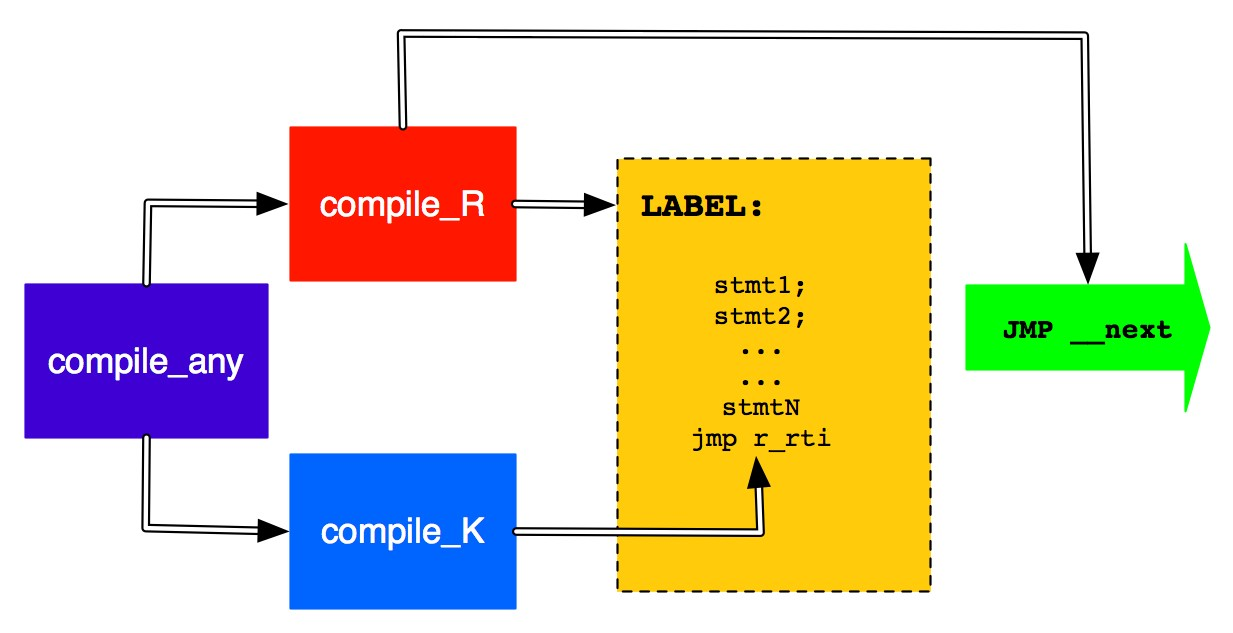
\includegraphics[height=5cm]{compilation_arch.jpg}}
\end{center}

\begin{itemize}

\item{Type annotations are used to separate terms by monadic type}

\item{Resumption-monadic terms are compiled to obtain label annotations, control flow transitions}

\item{State-monadic terms are compiled to obtain imperative code}

\end{itemize}

\end{frame}


%%%% slide
\begin{frame}{RSI: A Block-Based Imperative Language}

\begin{structure}{Internal Representation of RSI}

%\begin{onlinebox}{10cm}

\begin{tabular*}{10cm}[]{lc}
{
\begin{minipage}[t]{3.5cm}

\scriptsize{

$
\begin{array}[t]{lcl}

Code &::=& R \mid K\\
R &::=& Label\ Chain\\
K &::=& Label\ Block\\
Block &::=& Label\ ASM\\
\end{array}
$

}  % end fontsize

\end{minipage}
}

{
\begin{minipage}[t]{1.85in}

\begin{scriptsize}

$
\begin{array}[t]{lcl}

Chain &::=& Block\texttt{;}\ Chain\\
&\mid& Label\ \texttt{branch}\ Expr\ Label\\
&\mid& Label\ \texttt{jump}\ Ref\ Chain\\
&\mid& Label\ \texttt{halt}\\
\end{array}
$
\end{scriptsize}
\end{minipage}
}
\end{tabular*}

\medskip
\scriptsize
{\ \ \ \ \ $ASM ::= Stmt\texttt{;}\ ASM\ \mid \texttt{branch}\ Expr\ Block\ Block\ Block\ \mid \texttt{jump}\ Ref\ ASM$}
%\end{onlinebox}
\end{structure}

\medskip

\begin{structure}{Target: A Simplified Assembly Language (SAL)}

\medskip
\begin{onlinebox}{11cm}

\begin{scriptsize}
\begin{tabular}[]{ccccc}

\begin{minipage}[t]{3cm}
\texttt
{$Var$ := $Expr$\\
$Var$ := $Label$\\}
\end{minipage}

\begin{minipage}[t]{3cm}
\texttt
{bz $Expr$ $Label$\\
bz $Expr$ $Ref$\\}
\end{minipage}

\begin{minipage}[t]{3cm}
\texttt
{jmp $Expr$\\
jmp $Ref$\\}
\end{minipage}

\begin{minipage}[t]{1cm}
\texttt{nop\\
halt\\}
\end{minipage}

\end{tabular}
\end{scriptsize}

\end{onlinebox}

\end{structure}

\medskip

\begin{itemize}
\item{Program execution is specified as a $Chain$ of labeled $Block$s}
\item{Each block contains a sequence of simple assembly directives}
\item{Control flows among blocks according to their labels}
\item{RSI is readily transcribed to SAL in way that preserves semantics}
\item{\emph{How?}}
\end{itemize}

\end{frame}


%%%% slide
\begin{frame}{Representing the State Monad}

\begin{structure}{Characteristic Morphisms of the State Monad}

\smallskip

\begin{onlinebox}{9.5cm}
\begin{tabular}[]{cc}

\begin{minipage}{4cm}
$get\ ::\ StateT\ s\ m\ s$\\
$get = S\ (\lambda s . (s,s))$
\end{minipage}

\begin{minipage}{5cm}
$put\ ::\ s \rightarrow \ StateT\ s\ m\ ()$\\
$put\ x = S\ (\lambda \_ . ((),x))$
\end{minipage}

\end{tabular}

\end{onlinebox}
\end{structure}


\begin{itemize}
\item{State actions are expressible as simple assignments}
\item{Binding in the state monad reduces to sequencing assignments}
\end{itemize}

\bigskip

\begin{structure}{Compiling the Basic State Morphisms}

\smallskip

\begin{onlinebox}{7.75cm}
\begin{tabular}[t]{lll}
$
\begin{array}[t]{lll}
\lceil get_x \rceil_K &=& $\texttt{x := r\_ret}$\\
\lceil put_x\ v\rceil_K &=& $\texttt{x := v; r\_ret := CLEAR}$\\
\end{array}
$
\end{tabular}
\end{onlinebox}

\medskip

\begin{itemize}
\item{\texttt{r\_ret} is a distinguished reference corresponding to the monadic return value}
\item{\texttt{CLEAR} is a constant corresponding to the unit type, ()}
\end{itemize}

\end{structure}


\end{frame}


%%%% slide
\begin{frame}{Compiling the State Monad}

\begin{structure}{Compilation of State-Monadic Terms}
\begin{center}
\begin{onlinebox}{9cm}
\begin{tabular}[t]{lll}

%\begin{scriptsize}
$
\begin{array}[t]{lll}

\lceil k\ \bigstar_K\ \lambda v . k\prime\rceil_K &=& \lceil k \rceil_K $\texttt{; v := r\_ret;}$\ \lceil k\prime \rceil_K\\

\lceil \eta_K\ x\rceil_K &=& $\texttt{r\_ret := }$\ \lceil x \rceil_{any}\\

%\lceil v_{fun} \rceil_K &=& $\texttt{jmp }$ \mu(v)\\
\lceil v \rceil_K &=& \texttt{v\_back = BACK}\\
&&\texttt{jmp}\  \mu(v)\\
&&\texttt{BACK: nop}\\

\end{array}
$
%\end{scriptsize}

\end{tabular}
\end{onlinebox}
\end{center}
\end{structure}

\begin{itemize}

%\item{Bind produces sequencing, an intermediate assignment}

%\item{Identifiers declared at the top level produce jumps to the location of the corresponding compiled code, denoted $\mu$}

\item{$\mu$ denotes the location of compiled code of $v$ in the stored program's address space}

%\item{$\rho$ denotes the contents of $v$ in its current environment}

%\item{A variable produces a jump to an address determined by the binding of the variable in its current environment $\rho$}

\end{itemize}

\begin{structure}{Branching in the State Monad}
\begin{center}

\begin{onlinebox}{9cm}

%\begin{scriptsize}

\begin{tabular}[t]{llll}
$
\begin{array}[t]{llll}

\lceil if\ x\ then\ k\ else\ k\prime\rceil_K =& \texttt{bz}\ \lceil x \rceil_{Id}\ \texttt{L2}\\
&\texttt{L1:} \lceil k \rceil_K\texttt{; jmp}\ L3\\
&\texttt{L2:} \lceil k\prime \rceil_K\texttt{; jmp}\ L3\\
&\texttt{L3: nop}\\

\end{array}
$
\end{tabular}

%\end{scriptsize}

\end{onlinebox}
\end{center}

\end{structure}

\end{frame}


%%%% slide
\begin{frame}{Representing the Resumption Monad}

\begin{structure}{Characteristic Morphism of the Resumption Monad}

\begin{center}

\begin{onlinebox}{6.25cm}

\begin{flushleft}
$step\ ::\ m\ a \rightarrow ResT\ m\ a$\\
$step\ x\ =\ Pause\ (x\ \bigstar_m\ (\eta_m \circ \eta_R))$\\
\end{flushleft}

\end{onlinebox}

\end{center}

\end{structure}

\begin{itemize}

\item{$step$ specifies the entry point to a block of code, i.e. $Pause$}

\item{$step$ also specifies the entry point of the next block to execute, i.e. the $\bigstar_m\ (\eta_m \circ \eta_R)$}

\end{itemize}

\begin{structure}{Compiling $step$}

\begin{center}
\begin{onlinebox}{10cm}
\begin{flushleft}

\begin{tabular}[t]{llll}

$\lceil step\ x\ \bigstar_R\ \lambda v.\ x\prime \rceil_R =$&\texttt{PAUSE: r\_rti := PAUSE\_NEXT}\\
&\texttt{ST: r\_nxt := PAUSE\_NEXT}\\
&$\lceil x \rceil_K$\texttt{; jmp r\_rti}\\
&\texttt{PAUSE\_NEXT: }$\ \lceil x\prime \rceil_R$\\


\end{tabular}

\end{flushleft}
\end{onlinebox}
\end{center}

\end{structure}

\begin{itemize}

\item{\texttt{r\_ret} contains the value passed from $\lceil x \rceil_K$}
\item{\texttt{r\_rti} contains the location of the next action, $\lceil x\prime \rceil_R$}

\end{itemize}

\end{frame}


%%%% slide
\begin{frame}{Compiling the Resumption Monad}

\begin{structure}{Compilation of Resumption-Monadic Terms}

\begin{onlinebox}{9cm}

\begin{tabular}[t]{lll}

$
\begin{array}[t]{lll}

\lceil r \bigstar_R \lambda v.\ r\prime \rceil_R &=& \lceil r \rceil_R\texttt{; L: v := r\_ret;}\ \lceil r\prime \rceil_R\\

\lceil \eta_R\ x\rceil_K &=& $\texttt{L: r\_ret := }$\ \lceil x \rceil_{any}\\

%\lceil v_{fun} \rceil_R &=& \texttt{L: jsr}\ \mu(v)\\

%\lceil f_{var}  \rceil_R &=& \texttt{L: jsr}\ \rho(v)\\
\lceil r \rceil_K &=& \texttt{r\_back = BACK;}\\
&&\texttt{jmp}\  \mu(r)\\
&&\texttt{BACK: nop}\\

\end{array}
$

\end{tabular}

\end{onlinebox}

\end{structure}

\begin{itemize}

\item{Terms formed by binding, identifier reference are identical to those in state, except that each action is labeled}

\item{Note that, in a type-safe term, compile\_K will only be applied to K-typed code, compile\_R to R-typed code}

\end{itemize}

\begin{structure}{Branching Resumptions}
\begin{onlinebox}{9cm}

\begin{tabular}[t]{llll}
$
\begin{array}[t]{llll}

\lceil if\ x\ then\ r\ else\ r\prime\rceil_R =& \texttt{L0: bz}\ \lceil x \rceil_{Id}\ \texttt{L2}\\
&\texttt{L1:} \lceil r \rceil_R\texttt{; jmp L3}\\
&\texttt{L2:} \lceil r\prime \rceil_R\texttt{; jmp L3}\\
&\texttt{L3: nop}\\

\end{array}
$
\end{tabular}

\end{onlinebox}

\end{structure}

\end{frame}


%%%% slide
\begin{frame}{Twists on the Resumption: Loops and Breaks}

\begin{structure}{Compiling Loops}

\begin{onlinebox}{11cm}
$
\lceil loop\ (\lambda v.\ r) \rceil_R = \texttt{L: v:= r\_ret;} \lceil r \rceil_R\texttt{; jmp L; L\_EXIT: nop}
$
\end{onlinebox}

\end{structure}

\begin{itemize}

\item{$loop$ produces simple tail recursion, with a statically defined exit point}

\item{Loop variables are passed through \texttt{r\_ret}}

\end{itemize}

\begin{structure}{Compiling Break}

\begin{onlinebox}{10cm}

$
\lceil break\ v \rceil_R = \texttt{r\_ret :=} \lceil v \rceil_{Id} \texttt{; jmp L\_EXIT: nop}
$

\end{onlinebox}
\end{structure}

\begin{itemize}

\item{Compiler tracks which loop is currently in lexical scope}
\item{$break$ is simply a jump to the end of the enclosing loop}

\end{itemize}


\end{frame}


%%%% slide
\begin{frame}{Things Get Interesting}

\begin{center}
\structure{Slap that pig!}{
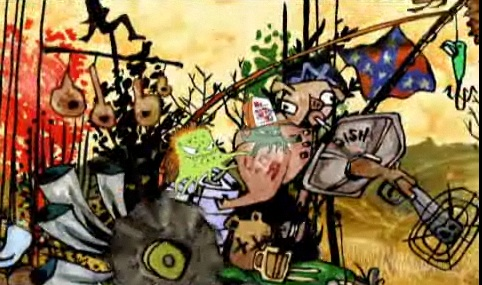
\includegraphics[height=5cm]{structure}}
\end{center}

\begin{itemize}

\item{Function application}

\item{Resumption deconstruction}

\item{A new morphism}

\item{Designer threads? Corner cases?}

\end{itemize}

\end{frame}


%%%% slide
\begin{frame}{Compiling Functions: CBV with Everything You See Here}

\begin{structure}{Call-by-Value Application: General Case}
\begin{onlinebox}{10cm}

\begin{tabular}[t]{llll}
$
\begin{array}[t]{llll}

\lceil f\ v\ \rceil_m &= &\texttt{x :=}\ eval (\lceil v \rceil_{any})\\
&&\texttt{f\_back := BACK}\\
&&\texttt{jmp }\mu(f)\\
&&\texttt{BACK: nop}&\ \{\lceil v \rceil_{any} \} \\
\end{array}
$
\end{tabular}

\end{onlinebox}
\end{structure}

\medskip

\begin{structure}{Function Declaration}
\begin{onlinebox}{9cm}

$\lceil f\ x\ = T\rceil_{dec} = \lceil T \rceil_{any}\texttt{; jmp f\_back}$

\end{onlinebox}
\end{structure}

\begin{itemize}

\item{The argument $v$ acts in two different capacities:}

  \begin{itemize}
  
  \item{As an expressible value assigned to the formal parameter $x$}
  
  \item{As a block of code emitted as part of the compiler output}
  
  \end{itemize}
  
\item{$eval$ produces the location of the beginning of $v$ when $v :: m\ a$, otherwise a simple expression}

\item{This general strategy will work for either monad but ... "product may vary from depiction"}

\end{itemize}

\end{frame}



%%%% slide (continued from last)

\begin{frame}{Compiling Functions: the Compiler Plays CBN}

\begin{structure}{Compiling Abstracted Monadic Actions: On-the-Spot Inlining}
\begin{onlinebox}{8cm}

\begin{tabular}[t]{lll}
$
\begin{array}[t]{lll}

\lceil (\lambda x.\ t)\ v \rceil_m& = \lceil \ t[x \mapsto v] \ \rceil_m \\

\end{array}
$
\end{tabular}

\end{onlinebox}
\end{structure}

\medskip

\begin{structure}{Okay ...}
\begin{itemize}

\item{Greatly simplifies compilation, and hence verification}

\item{It is tractable to compile applications $:: m\ a \rightarrow m\ b$, but this requires invoking some bad magic, angering the proof-gods}
\begin{itemize}\item{If you want to be technical, passing and repeatedly reffing/de-reffing pointers to jump-back variables through a chain of calls}\end{itemize}

\end{itemize}
\end{structure}

\pause

\begin{structure}{... But There's a Downside}

\begin{itemize}
\item{Most interesting kernel behaviors involve functions with monadic arguments}
  \begin{itemize}
  \item{$handler\ ::\ Re\ a \rightarrow R\ a$}
  \item{$sched\ :: Re\ a \rightarrow Re\ a \rightarrow R\ a$}
  \end{itemize}
  
\item{Arguments to $sched$ and $hand$ cannot in general be inlined}
\begin{itemize}\item{If they could, there would be nothing for the kernel to do!}\end{itemize}
\item{Real problem: handling effective jump-back from a resumption}
\end{itemize}


\end{structure}

\end{frame}


%%%% slide

\begin{frame}{Call Stacks: Another Dire Warning About a Minor Issue}

\forget{
\begin{structure}{It's Not Just State!}

\begin{onlinebox}{11cm}

\begin{scriptsize}
\begin{flushleft}


\texttt{nextof :: R a $\rightarrow$ R (R a)}
\texttt{nextof r =}\\
\texttt{\ \ case r of}\\
\texttt{\ \ (Pause k) -> step\_R k}\\
\texttt{\ \ (Done v) -> step\_R r}\\
\ \\
\texttt{main =}\\
\texttt{\ \ loop ($\lambda$(r1, r2) ->}\\
\texttt{\ \ \ \ if (done r1) then break () else nextof r1 >>= $\lambda$r3 -> return (r2, r3))}\\

\end{flushleft}
\end{scriptsize}

\end{onlinebox}

\end{structure}

\begin{structure}{Something to Think About}
\begin{itemize}

\item{\texttt{leave} produces a new resumption by punctuating the actions of \texttt{r2} with the next action of \texttt{r1}}


\end{itemize}
\end{structure}

} % end forget

\begin{structure}{We Can Inline This ...}

\begin{center}

\begin{onlinebox}{7cm}

\begin{scriptsize}

\texttt{main = step\_R x >> (nest r0)>> step\_R y}\\
\ \\
\texttt{nest r = step\_R x >> (r0 r) >> step\_R y}\\
\texttt{r0 r = step\_R x >> (r1 r) >> step\_R y}\\

$\cdots$

\texttt{rM r = step\_R x >> (rN r) >> step\_R y}\\

\texttt{rN r = step\_R x >> r >> step\_R y}\\

\end{scriptsize}

\end{onlinebox}\end{center}\small{Since all references to monadic args can be resolved at compile-time!}

\end{structure}

\smallskip

\begin{structure}{... But Not This}

\begin{center}
\begin{onlinebox}{8cm}

\begin{scriptsize}
\begin{flushleft}

\texttt{main = loop ($\lambda$r -> nest (step\_R (nextof r)))}\\
\ \\
\texttt{nextof r =}\\
\texttt{\ \ case r of}\\
\texttt{\ \ \ \ (Pause x) -> step\_R x}\\
\texttt{\ \ \ \ (Done v) -> step\_R (return v)}\\

\end{flushleft}
\end{scriptsize}

\end{onlinebox}
\end{center}

\end{structure}
\small{Because the argument to \texttt{main} has to be run through completely!}\\
\color{red}{\small{\emph{We can, however, inline} \texttt{nextof} \emph{and} \texttt{nest}}}


\end{frame}

%%%% slide

\begin{frame}{An Interesting Conjecture}

\begin{large}

\begin{center}
\begin{structure}{What kind of thing has this type?}


$t :: R\ a \rightarrow\ R\ a$

\end{structure}
\end{center}
\end{large}


\pause

\center{\emph{\large{\color{red}{It's a thread!}}}}

\medskip

\begin{structure}{Threads with 'pthreads' in C}

\begin{onlinebox}{10cm}

\begin{small}
\begin{flushleft}

\texttt{\ \ \ \ t = (pthread\_t*) malloc(sizeof (pthread\_t);}\\
\texttt{\ \ \ \ pthread\_create(t, NULL, foo, (void*) arg);}\\
\texttt{\ \ \ \ pthread\_join(t, retcode);}\\
\ \\
\texttt{\ \ \ \ int foo(void* arg)\{ ... \}}\\

\end{flushleft}
\end{small}

\end{onlinebox}
\end{structure}

\medskip

\begin{structure}{"Joining" a Thread in CT}

\begin{onlinebox}{9cm}

\begin{flushleft}

\texttt{\ \ \ \ join t r = init >> t >>= $\lambda$arg -> r}\\
\texttt{\ \ \ \ init = put$_{arg}$ thread\_argument}\\

\end{flushleft}
\end{onlinebox}

\end{structure}

% begin forget:
\forget{

\begin{itemize}

\item{A thread is a "lightweight process" without its own address space}

\item{A process, by definition, runs in the midst of some enveloping execution stream}

\item{That means, given some other execution stream $r$, $t$ denotes the execution of thread $t$ relative to $r$}

\item{In particular, both $sched$ and $handler$ are proper threads according to this definition}

\item{Compare with usages of the pthreads library in C, esp. the use of 'pthread\_join'}

\item{\emph{Can we characterize the notion of threads in terms of this type?}}


\end{itemize}
} % end forget



\end{frame}


%%%% slide
\begin{frame}{Good News: A Persistent Issue, Finally Resolved}

\begin{structure}{Deconstructing Resumptions, Atom by Atom}
\begin{onlinebox}{8cm}
\begin{flushleft}
\smallskip

\texttt{\scriptsize
{nextof :: R a -> R (R a)\\
nextof r =\\
\ \ case r of\\
\ \ \ \ (Pause x) -> step\_R x >>= $\lambda$r -> return r\\
\ \ \ \ (Done v) -> step\_R (return v)
}}

\end{flushleft}
\end{onlinebox}
\end{structure}

\begin{itemize}

\item{Exactly the first action of \texttt{r} should run}
\item{After the first action is run, a reference to the rest of \texttt{r} should be passed to the return value}

\end{itemize}

\pause

\begin{structure}{Compiled!}

\smallskip

\begin{tabular}[t]{llll}

$
\begin{array}[t]{llll}

\lceil \texttt{(Pause x) -> step\_R\ x}\rceil_R =& \texttt{x := r + PAUSE\_HEADER}\\
&\texttt{r\_rti := L; jmp x}\\
&\texttt{L: r\_ret := r\_nxt}

\end{array}
$
\end{tabular}

\end{structure}

\end{frame}


%%%% slide
\begin{frame}{Compiling Resumption Deconstruction}

\begin{structure}{Atom Shuffling Via Jumps}
\begin{onlinebox}{9cm}
\begin{tabular}[t]{llll}

\begin{scriptsize}
$
\begin{array}[t]{llll}

\lceil \texttt{(Pause x) -> step\_R\ x}\rceil_R =& \texttt{x := r + PAUSE\_HEADER}\\
&\texttt{r\_rti := L; jmp x}\\
&\texttt{L: r\_ret := r\_nxt}

\end{array}
$
\end{scriptsize}
\end{tabular}
\end{onlinebox}
\end{structure}

\bigskip

\begin{structure}{How It Works: Using the Definition of $step$}

\begin{onlinebox}{10cm}
\begin{flushleft}

\begin{scriptsize}
\begin{tabular}[t]{llll}

$\lceil step\ x\ \bigstar_R\ \lambda v.\ x\prime \rceil_R =$&\texttt{PAUSE: r\_rti := PAUSE\_NEXT}\\
&\texttt{ST: r\_nxt := PAUSE\_NEXT;}$\lceil x \rceil_K$\texttt{; jmp r\_rti}\\
&\texttt{PAUSE\_NEXT: }$\ \lceil x\prime \rceil_R$\\


\end{tabular}
\end{scriptsize}

\end{flushleft}
\end{onlinebox}

\begin{itemize}

\item{Each atom is suffixed by a jump determined by \texttt{r\_rti}}
\item{Deconstruction bypasses the initial assignment to \texttt{r\_rti} at \texttt{PAUSE}, goes to start of state code at \texttt{ST} instead}

\begin{itemize}
\item{\scriptsize{\texttt{PAUSE\_HEADER} is a fixed-size offset determined by the footprint of the initial assignment to \texttt{r\_rti}}}
\end{itemize}

\item{When \texttt{jmp r\_rti} is reached at the end of $\lceil step\ x\rceil$, control flows back to invoking resumption at \texttt{L}}

\end{itemize}

\end{structure}

\end{frame}


%%%% slide

\begin{frame}{Introducing \texttt{resume}}

\begin{structure}{The Atom-Smashing Morphism}
\begin{onlinebox}{9cm}

\begin{tabular}[t]{lll}
$resume$ &$::$ $R\ a \rightarrow R\ (R\ a)$\\
$resume\ r\ $&$\equiv \ \ case\ r\ of$\\
&$\ \ \ \  \ \ (Pause\ x) \rightarrow step_R\ x$\\
&$\ \ \ \ \ \ (Done\ v) \rightarrow step_R\ ((\eta_K\ \circ \eta_R)\ v)$\\

\end{tabular}

\end{onlinebox}
\end{structure}


\begin{itemize}

\item{$resume$ provides a CT-source primitive for deconstructing resumptions}

\item{Virtually all interesting kernels involve deconstruction, which justifies a primitive}

\item{A well-defined primitive provides simpler source code and more economical compilation, e.g. this one-line kernel:}
\end{itemize}

\begin{structure}{hello world}
\begin{onlinebox}{11cm}

\begin{scriptsize}

\texttt{main = loop ($\lambda$(r1, r2) -> resume r1 >>= $\lambda$r3 -> return (r2, r3))}

\end{scriptsize}

\end{onlinebox}
\end{structure}


\end{frame}



%%%% slide
\begin{frame}{Fun with CT: Pushing the Limits}

\begin{structure}{Arbitrary Code Insertion}

\begin{onlinebox}{11cm}

\begin{scriptsize}
\begin{flushleft}

\begin{texttt}
\texttt{punct :: K a $\rightarrow$ R a\\}
\texttt{punct act = loop ($\lambda$r -> if (done r) then r else step\_R(act >> atom r))}\\
\end{texttt}

\end{flushleft}
\end{scriptsize}

\end{onlinebox}
\end{structure}


\begin{structure}{Thread Counting}

\begin{onlinebox}{11.5cm}

\begin{scriptsize}
\begin{flushleft}

\texttt{threadct :: R a $\rightarrow$ Int}\\
\texttt{threadct = loop ($\lambda$(r, n) -> if (done r) then break n else (rtail r, n + 1))}\\

\end{flushleft}
\end{scriptsize}

\end{onlinebox}

\end{structure}


\begin{center}

\begin{structure}{Reverse-Sequencing Actions}
\begin{onlinebox}{9cm}

\begin{scriptsize}
\begin{flushleft}

\begin{texttt}
\texttt{reverse :: R a $\rightarrow$ R a\\}
\texttt{reverse r =}\\
\texttt{\ \ (loop ($\lambda$(k, t) ->\\
\ \ \ \ if (done t) then break k\\
\ \ \ \ else step\_R(atom t) >>= $\lambda$s -> return (s >> k, nextof t)}\\
\texttt{\ \ ) r) >>= $\lambda$k -> step\_R k}
\end{texttt}

\end{flushleft}
\end{scriptsize}


\end{onlinebox}
\end{structure}


\end{center}


\end{frame}

%%%% slide
\begin{frame}{Things to Think About}

\begin{itemize}

\item{CT has first-class monadic actions, which allows for constructing new actions at runtime.
\begin{itemize}\item{What capabilities does this provide the programmer?} \item{What verification challenges does this pose?}\end{itemize}}

\smallskip

\item{Arguments to basic kernel services, e.g. $sched$ and $handler$, cannot, in general, be inlined.  \begin{itemize}\item{What programs can we write without being forced to fall back on the voodoo of indirect reference?}\item{Are these sufficient for our result to have the force we want?}\end{itemize}}

\item{Is it possible to tweak the inlining procedure in a way that removes the complications of function application without producing huge code?}

\item{Is the control flow for a CT program decidable?
\begin{itemize}\item{I'm pretty sure it is} \item{Can it be leveraged into an even more powerful verification?}\item{Does this present the opportunity for tractable dynamic monitoring?}\end{itemize}}

\end{itemize}

\end{frame}

%%%% slide
\begin{frame}{Questions?}

\begin{center}
%
\includegraphics[height=5cm]{thanks}

\includegraphics[height=6cm]{looked_different}

\structure{"Damn!  You looked different in the denotational semantics!"}

\end{center}

\end{frame}

\end{document}
